\documentclass[letterpaper,10pt,notitlepage]{report}
\usepackage[left=1in,top=1in,right=1in,bottom=1in,nofoot]{geometry}
\usepackage{alltt}
\usepackage{listings}
\usepackage{amsmath}
\usepackage{fancyhdr}
\usepackage{textcomp}
\usepackage{graphicx}
\usepackage{indentfirst}
\usepackage{setspace}
\usepackage[normalem]{ulem}
\pagestyle{fancy}
\lhead{\thepage{}}
\rhead{Joseph Colosimo \:\:\: 6.115 \: Final Project}
\cfoot{}

\newenvironment{code}{\begin{quote}\begin{alltt}}{\end{alltt}\end{quote}}
\newcommand{\projname}{\texttt{Cerebro}}

\setstretch{0.95}

\setcounter{secnumdepth}{3}
\def\thesection{\arabic{section}}
\def\thesubsection{\arabic{section}.\arabic{subsection}}
\def\thesubsubsection{\arabic{section}.\arabic{subsection}.\arabic{subsubsection}}

\begin{document}

\begin{center}
	\begin{huge}
		\textbf{\projname{} --- A Brainwave Visualizer}
	\end{huge}
\end{center}

\section{Background Motivation}
    I have many interests related to signal processing.  I have done a good 
    deal of audio processing both in the context of audio waveform 
    modification (e.g. high speed hardware parametric equalizers) and in music 
    visualization.  In trying to branch out from this interest, I have sought 
    other waveforms to examine and work with.  One such waveform is the 
    electromagnetic activity of the brain's surface.

    In late 2010, a company named NeuroSky began producing low-cost,
    single-sensor EEG chips.  These chips would read input from a sensor
    mounted to the forehead and two reference pads clipped to the ears and
    amplify electromagnetic signals from the surface of the brain while
    eliminating background noise.  The chip contains a built-in FFT block that
    reads the waveform and produces relative power values of frequency bands
    defined by neuroscience.  Furthermore, the chip computes ``attention'' and
    ``meditation'' values --- empirical values representative of user's state
    of mind.

    This chip has been employed in various devices and is generating 
    interest in the neuroscience field because it provides a low-cost 
    method for analyzing basic electromagnetic activity of the brain.
    Additionally, one of the first commercial demonstrations of the product was performed by 
    Mattel, who created a toy whereby the user would alter his or her level of 
    concentration to raise or lower a ball, moving it through an obstacle course.

    Having already hacked this toy to pull out the EEG data from 
    NeuroSky's chip, I have become interested in visualizing this data 
    on an LED-based lighting system.  This past January, I was the principle 
    electronics designer of a large lighting system that I built for my dorm.  
    We built several instruments, but one of them was a large,  24-``pixel'' 
    array of high powered red-green-blue (RGB) LEDs.  I intend to visualize 
    brainwave data on a 4-``pixel'' segment of this system (as seen in 
    Figure \ref{fig:photo}).

    \begin{figure}[h!]
    \begin{center}
        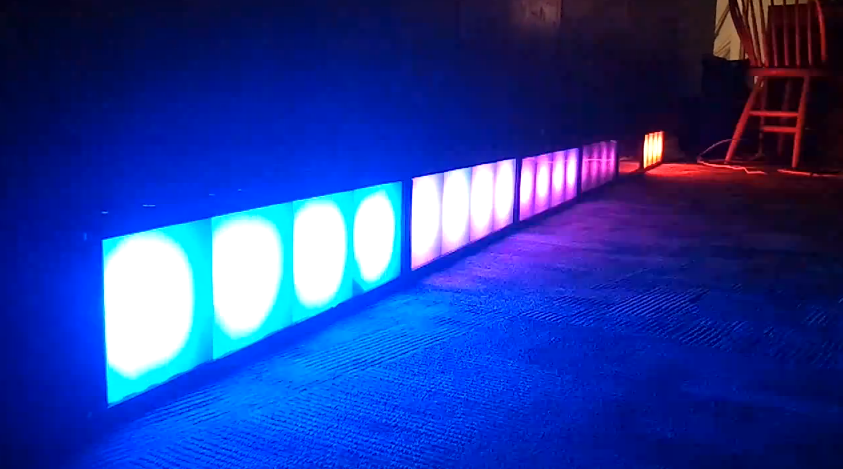
\includegraphics[scale=.2]{fig/photo.png}
        \caption{Segments of the front panel instruments from the Next House 
        Party Lighting System}
        \label{fig:photo}
    \end{center}
    \end{figure}

    I will create a custom algorithm for processing the brainwave data to 
    generate visual output on the panel.  Furthermore, I will use an analog 
    slider board taken from an equalizer to fine-tune processing parameters 
    and modify the operation of the algorithm.

\section{Hardware Interfaces}
    Figure \ref{fig:hw} describes \projname's hardware layout.

    \begin{figure}[h!]
    \begin{center}
        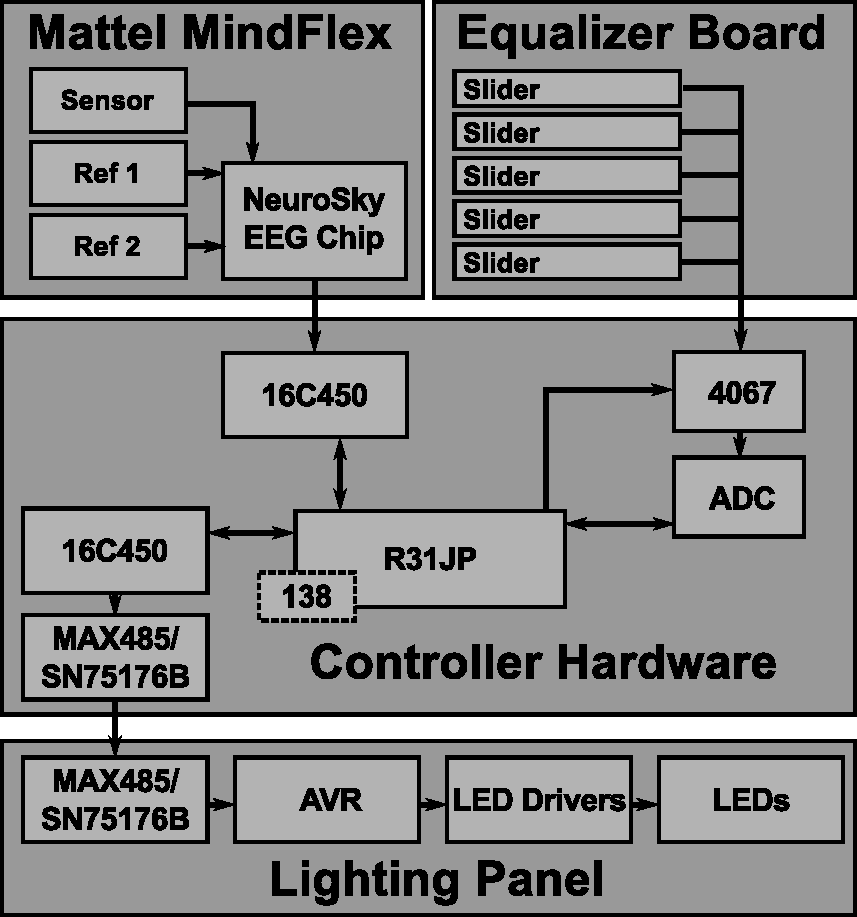
\includegraphics[scale=.4]{fig/blockdiagram.pdf}
        \caption{\projname{}'s overall hardware architecture.}
        \label{fig:hw}
    \end{center}
    \end{figure}

    \subsection{Mattel Mindset / NeuroSky EEG Chip Interface}

    While NeuroSky offers development kits, it is cheaper to purchase one of 
    Mattel's MindFlex toys and read data from the NeuroSky chip located in its 
    headband.  I purchased one of these toys, took apart the headband, and 
    modified the board slightly to receive transmitted data from the NeuroSky 
    chip's UART.%
        \footnote{http://company.neurosky.com/how-to-hack-toy-eegs-frontier-nerds-an-itp-blog/}
    Afterward, I was able to receive data packets from the EEG.

    The EEG uses TTL-level signals, so it is easy to interface to the 8051 
    through a 16C430 chip.
    
    \subsection{Equalizer Board Interface}

    A while ago, I purchased for \$6 a board containing a large number of 
    variable resistor sliders from a surplus electronics store.  This board 
    was originally used in a high end equalizer.  The board creates resistor 
    dividers out of all of the potentiometers and places the output pins onto 
    contacts on the back of the board.  So, using a methodology similar to 
    that of SpinDude, it is very easy to read the relative values of all resistors.

    The board has around 48 sliders, but I will only address 16 because I 
    don't anticipate needing more than this.  A 4067 analog multiplexer allows 
    the 8051 to select a slider output and pass its value to an ADC (likely 
    the ADC0801), which will send its output to the 8051.  The 8051, 
    therefore, can quickly scan through all of the sliders to obtain 
    values.  Powering the board is simply a matter of applying 5V and 
    ground to two terminals.

    \subsection{Lighting System Interface}

    I am part of a small student group called Next Make.  Our group's main 
    goal is to emphasize the engineering processes of design and construction 
    among students by working on various kinds of projects.  Throughout 
    January, we designed and built a large lighting system that has a variety of 
    instruments.  We use our own serial protocol (similar 
    to DMX) to send data to these devices over a high-speed RS-485 network.  
    We use a SN75176B (TI's cheaper equivalent of the MAX485) to convert the 
    RS-485 levels to TTL, feed this data into an Atmel ATMEGA168 which 
    processes the packets it receives and constructs a serial stream to send 
    over high speed SPI to TI's TLC5940 constant current sink PWMing LED 
    drivers.  We have posted videos of our early attempts%
        \footnote{http://www.youtube.com/watch?v=bPlrKSYWWJs}
    as well as a few of our final instruments%
        \footnote{http://www.youtube.com/watch?v=Wyv3h0ii2uI} that are 
    currently fully operational.

    Normally, the system is controlled by a computer performs realtime audio 
    processing.  I designed the boards and the microcontroller software and so I 
    plan to use one of the lighting instruments as the visualization interface 
    for this project.  A 16C430 will send its output to a MAX485 or SN75176B, 
    which will generate RS-485-level signals that will be sent to the panel 
    via an ethernet cable.  

\section{Software Design}
    Figure \ref{fig:sw} describes the overall flow of data through \projname's 
    software.

    Input interfaces are handled in a non-linear manner.  The interrupt pin of 
    the EEG's 16C450 is connected to one of the external interrupts of the 
    8051 so that with each received byte, the software invokes the packet 
    processor to continue processing a packet.  Likewise, the interrupt pin of 
    the ADC is connect to the other external interrupt pin of the 8051.  When 
    the ADC has finished processing data, the equalizer processor should use 
    the values to configure the signal processor.

    \begin{figure}[h!]
    \begin{center}
        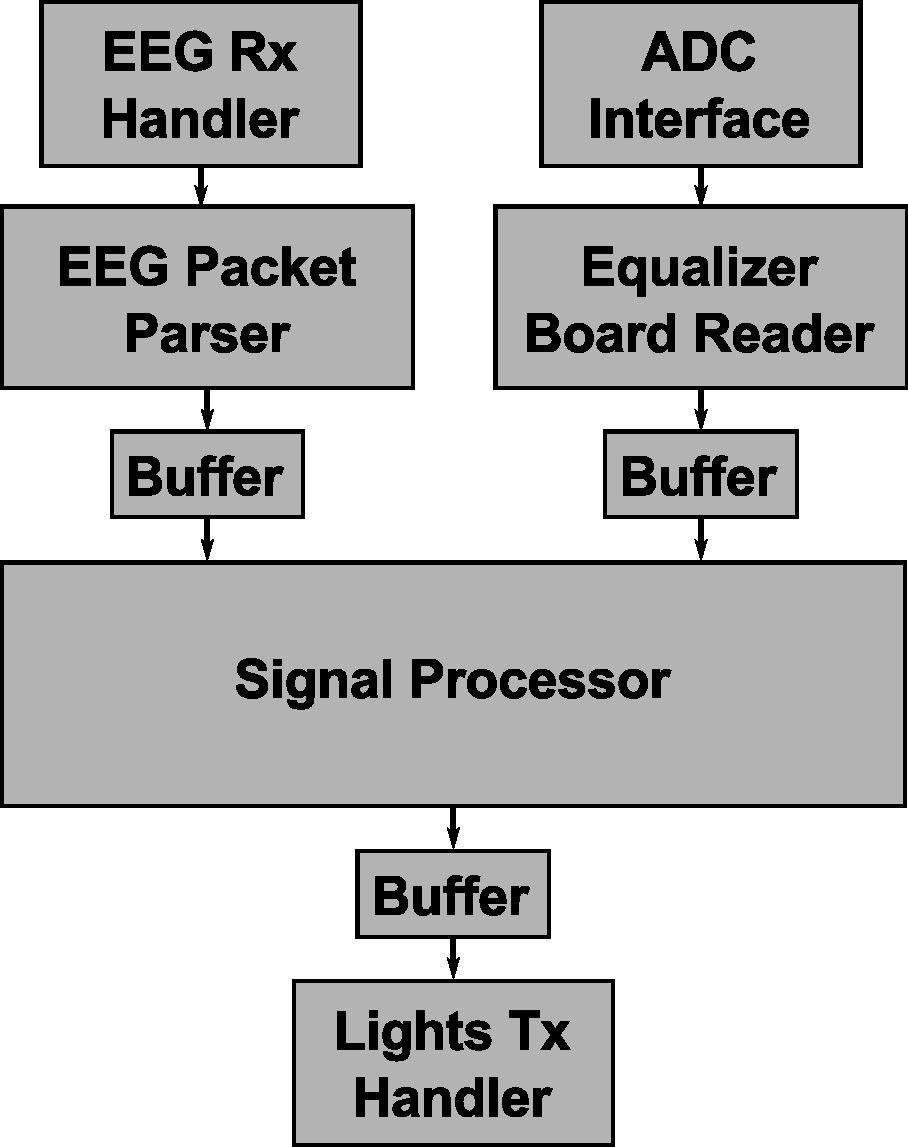
\includegraphics[scale=.3]{fig/software.pdf}
        \caption{\projname{}'s software flow.}
        \label{fig:sw}
    \end{center}
    \end{figure}

    \subsection{NeuroSky Packet Processor}
        NeuroSky publishes protocol documentation as well as some sample 
        packet processing algorithms.%
            \footnote{http://weartel.com/ece1766/mindset\_communications\_protocol.pdf}
        I partially implemented the processing protocol for the Atmel AVR in 
        order to investigate the chip's operation.  One of my first tasks will 
        be to translate this C code to 8051 assembly so that I can achieve 
        functionality with the labkit.

        When the 16C430 interrupts the processor, the packet processing system 
        will use its internal state machine process a packet according to 
        NeuroSky's protocol.  It will then place the parsed data (FFT power 
        values) into a buffer for the signal processor to use.

    \subsection{Equalizer Board Reader}
        The equalizer board reader will be on a slow timer.  Much like 
        SpinDude's method of operation, the software will scan through all of 
        the potentiometers and read their analog values, storing them in a 
        buffer for the signal processor.

    \subsection{Signal Processor}

        The bulk of this project is the design and implementation of a signal 
        processing algorithm that provides a ``visualization'' of brain 
        activity.  I have experience with audio signal processing and intend 
        to work based on some of the algorithms I have designed for multiband 
        visualizations in audio.  The EEG outputs FFT power values at 8 
        frequency bands; the relative powers of these bands are indicative 
        of the user's current activity, so an algorithm could, for example, 
        choose a hue based on this state.  Furthermore, the algorithm could 
        use the ``attention'' value from the EEG chip to determine the 
        brightness of the display output.

        I have several algorithms in mind, but my first goal is to start 
        reading of data from the headset in order to get an idea of what 
        kind of control system I can create from the headset data.
        
    \subsection{Lighting System Driver}
        
        After the signal processor block is done, it saves a final set of 
        color values for the display to a buffer and invokes the display 
        driver.  This driver assembles packets and sends it via the 16C430.

\section{Project Scope}
    This project is based around the construction and integration of several 
    distinct modules: the EEG processor, the equalizer processor, the lighting 
    system driver, and the signal processing algorithm.

    I envision a ``B'' grade project to be one where I implement a very simple 
    signal processor that adjusts the brightness of the light system based on 
    the user's level of attention.  The hue of each pixel will be controlled 
    by the sliders on the equalizer board.  This algorithm is extremely simple 
    to implement.  It would use the NeuroSky's ``attention'' composite value 
    (in fact, the whole packet processor can be simplified to search for just 
    this value) and set the hue by reading 12 equalizer sliders.  If the 
    equalizer board is not operational by the end of the project, I could 
    easily implement a hue cycling algorithm.

    An ``A'' level project will implement all of the hardware components as 
    well as a significant processing algorithm that uses all of the frequency 
    bands of the EEG to create a well-defined control system.  An EEG with a 
    single sensor can provide a large amount of data, but the most difficult 
    aspect of this project will be to design an algorithm that takes this data 
    and turns it into a meaningful control system for the lighting system.  
    Likewise, the equalizer board should provide a way of fine-tuning the 
    processing algorithm (for example, to determine the relative weights of 
    the frequency bands during processing).  Furthermore, an ``A'' level 
    project could provide multiple signal processing algorithms.  Perhaps they 
    could be selected with the keypad.

    A far more complex project would be to use multiple EEG sensors to read 
    several areas of the brain surface.  Studies utilizing 3-5 sensors have 
    been able to control complicated systems requiring thoughts like ``left'' 
    and ``right'' and it would be interesting to implement a system that 
    processes data from multiple EEGs.  This would require updates to the 
    signal processing algorithm as well as the creation of a modified headband 
    from several of Mattel's MindFlex toys.  I do not really want to pay for 
    multiple toys though, so I would have to find money elsewhere for it.  
    Alternatively, given that NeuroSky is actively seeking partnerships with 
    educational institutions, it might be able to provide me with free or 
    discounted chips and sensors.  I will investigate this avenue early in 
    case I have time to work on such a system.

\section{Required Components}
    I have already purchased and modified a Mattel MindFlex and have proven its 
    operability.  I also have a panel of the lighting system and its power supply.

    I will need the following components to complete my system:

    \begin{table}[h!]
    \begin{center}
        \caption{List of required electronics components}

        \begin{tabular}{|c|c|c|c|}
            \hline
            \textbf{Part} & \textbf{Qty. Req'd} & \textbf{Qty. in Labkit} & 
            \textbf{Add'l Qty. Needed} \\
            \hline
            ADC0801 & 1 & 1 & 0 \\
            \hline
            74LS138 & 1 & 1 & 0 \\
            \hline
            16C430  & 2 & 1 & 1 \\
            \hline
            4067 & 1 & 0 & 1 \\
            \hline
            SN75176B & 1 & 0 & 0 \\
            \hline
        \end{tabular}
    \end{center}
    \end{table}

    In summary, I will need one 16C430 and one 4067 to complete my design.  I 
    have a SN75176B.

\section{Timetable}
    I am somewhat ahead of schedule.  I was able to capture and 
    analyze data from the EEG.  Figure \ref{fig:eeg} shows the setup thus far.  
    Initial data from the EEG has show that sensor placement is critical, so I 
    will need to pay close attention to the signal quality information coming 
    from the EEG.  I have captured quite a bit of data so far to prove the 
    operability of the system; see Figure \ref{fig:braindump} for a graph 
    showing an example capture.

    \begin{figure}[h!]
    \begin{center}
        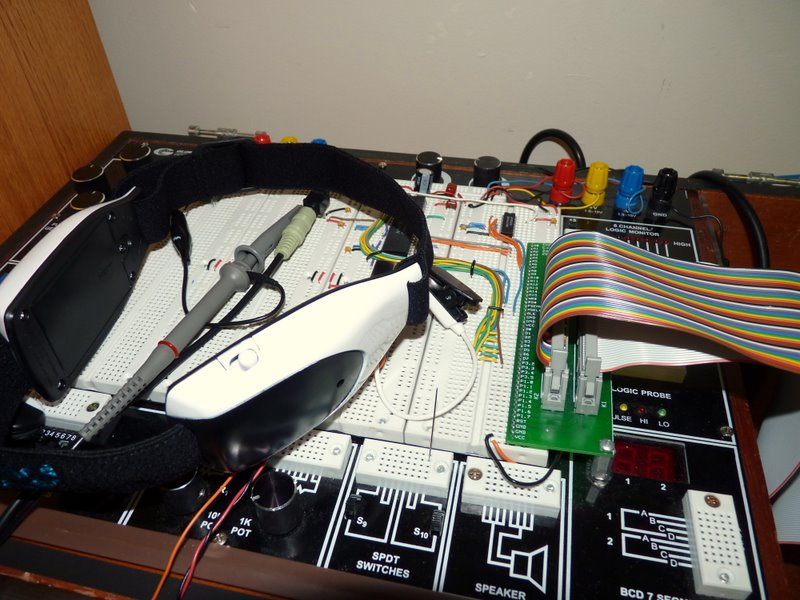
\includegraphics[scale=.25]{fig/photo2.jpg}
        \caption{EEG Setup}
        \label{fig:eeg}
    \end{center}
    \end{figure}

    \begin{figure}[h!]
    \begin{center}
        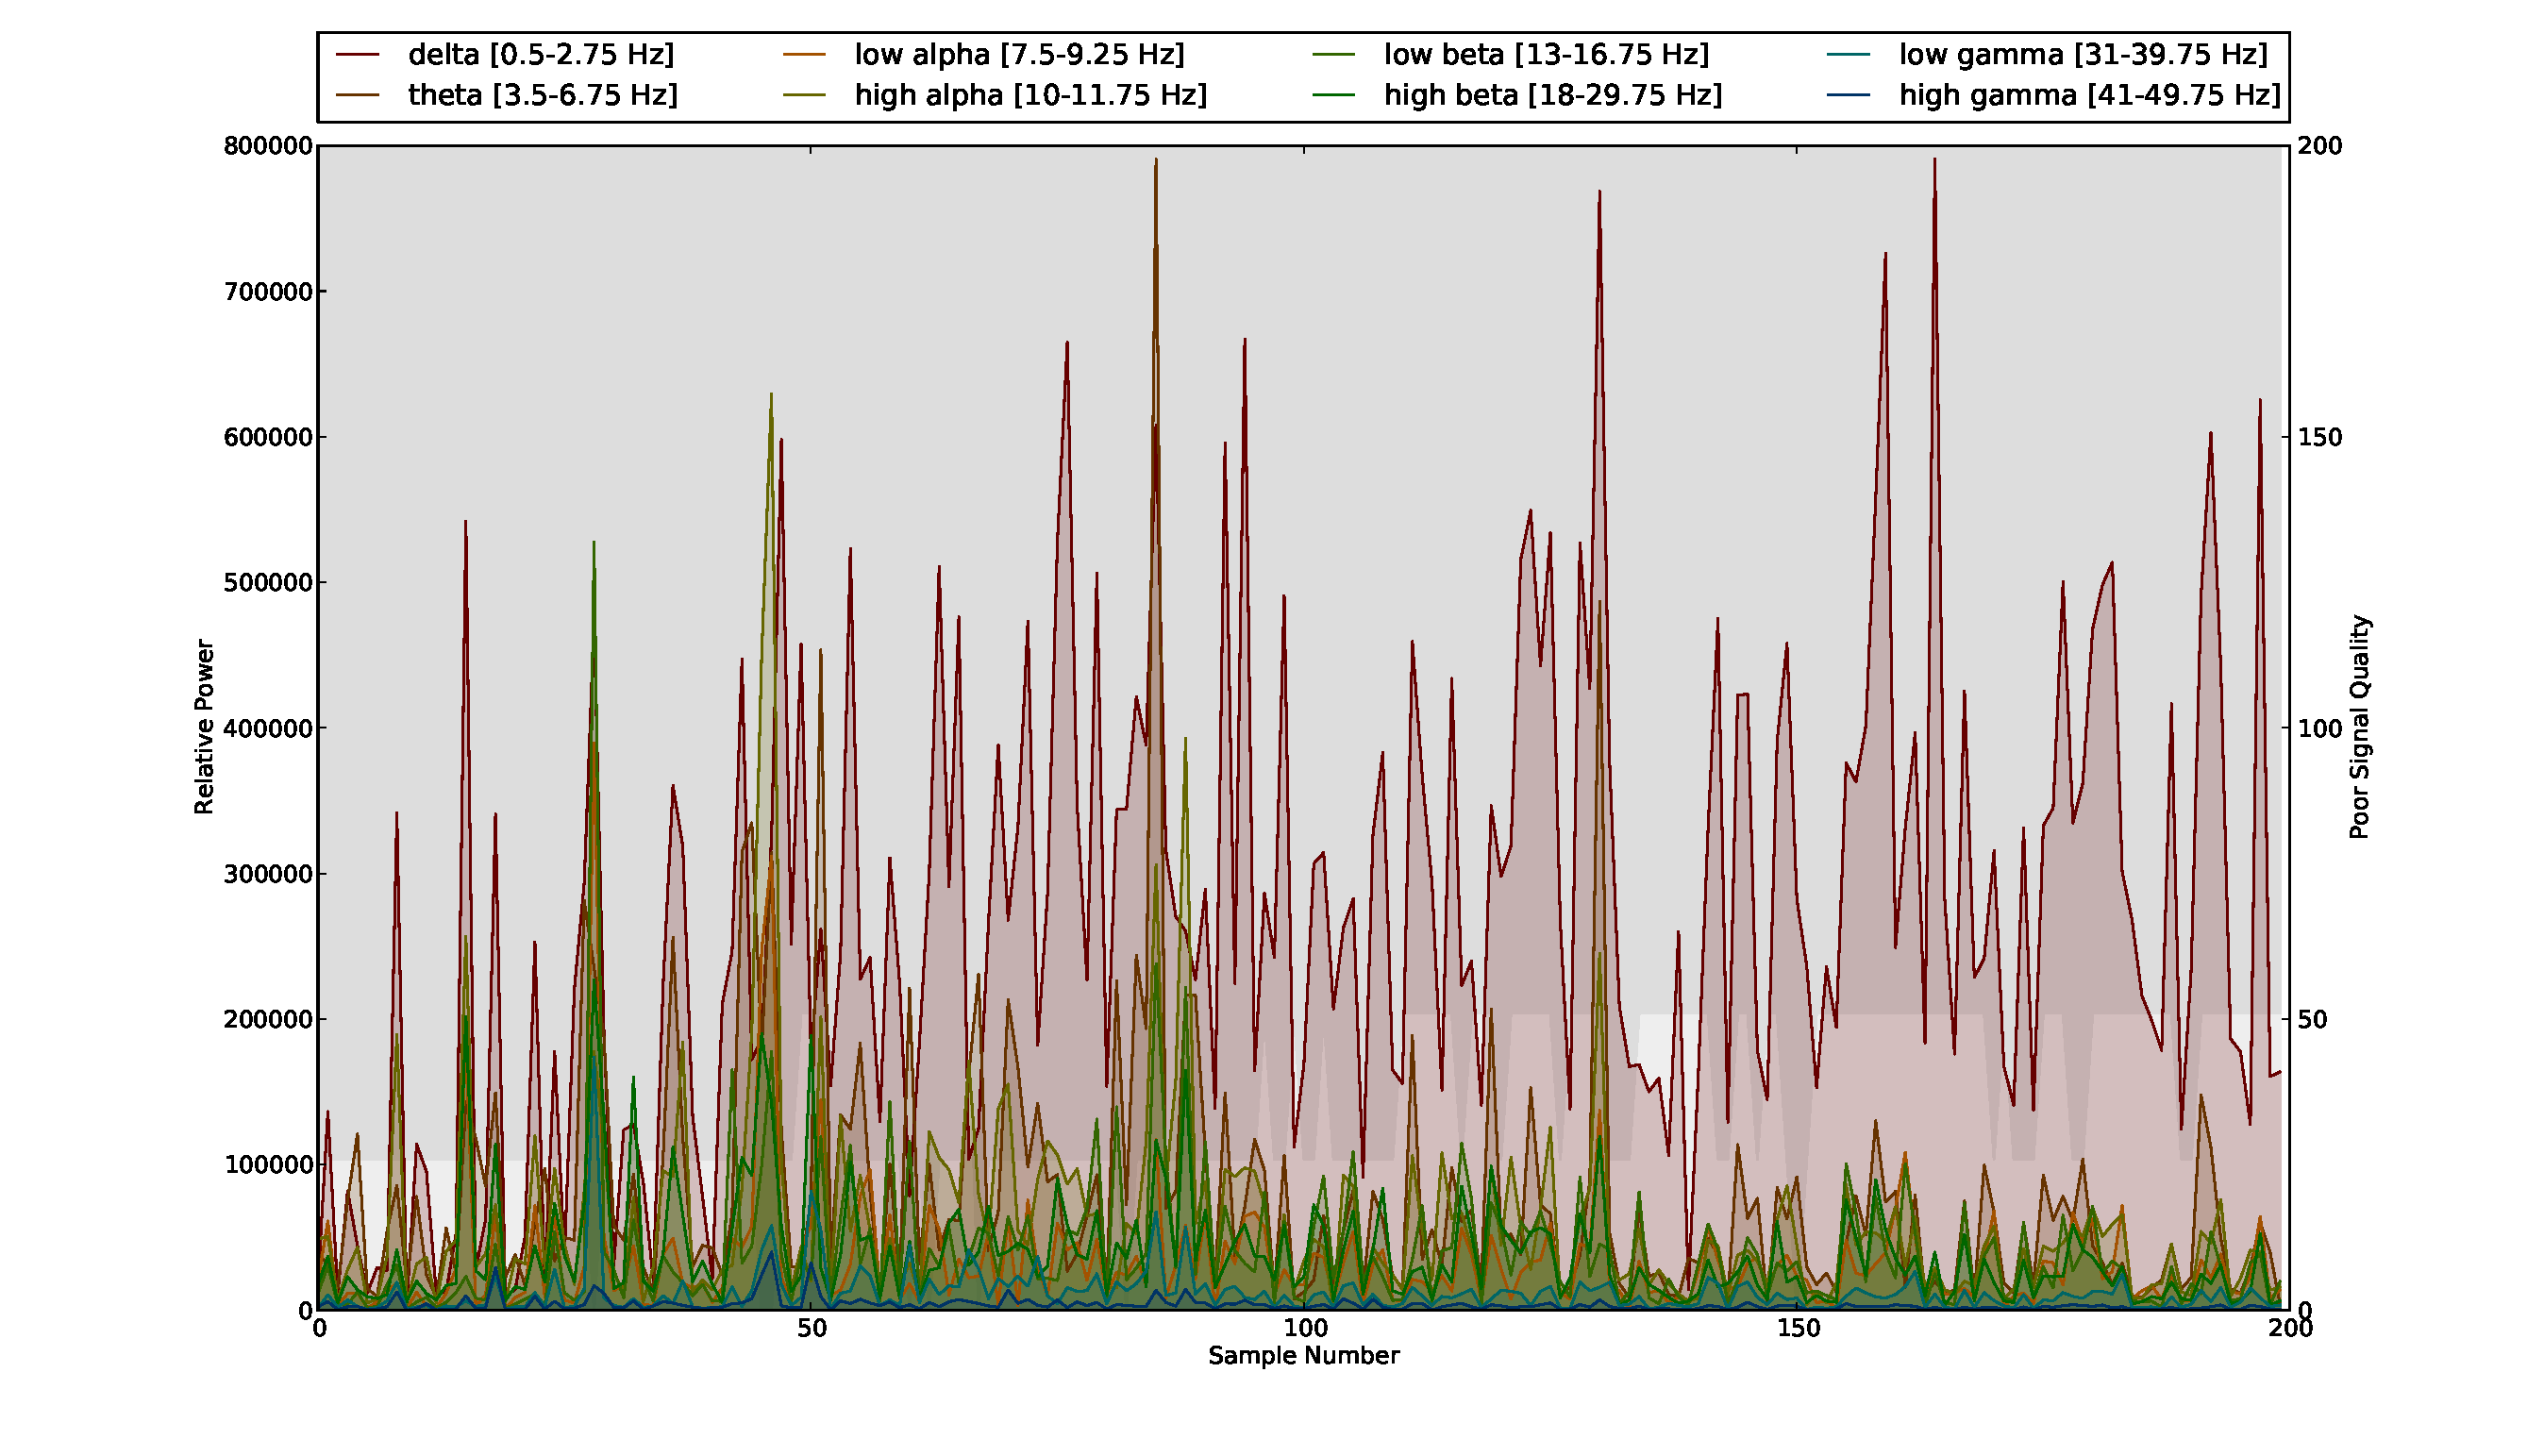
\includegraphics[scale=.35]{fig/braindump6.pdf}
        \caption{Example data captured from the EEG}
        \label{fig:braindump}
    \end{center}
    \end{figure}

    The lighting system is ready for interfacing with the Labkit.  I haven't 
    had a chance to start setting up the equalizer board, but I am not 
    planning to work on it until the other systems are up and running.

    A timetable describing how I plan to complete the remaining tasks follows.

    \subsection{April 18}
        \begin{itemize}
            \item Capture data to determine a good candidate algorithm for 
                  signal processing (send data via serial and graph it).
            \item Design math for at least one processing algorithm.
            \item Using recorded data, perform a simulation with the algorithm.
        \end{itemize}

    \subsection{April 25}
        \begin{itemize}
            \item Create the lighting system driver.
            \item Implement and test the signal processing algorithms designed 
                  in the previous week.
            \item If there is time, implement additional algorithms.
        \end{itemize}

    \subsection{May 2}
        \begin{itemize}
            \item Wire up equalizer board and write software to test its operability.
            \jtem Add controllable gains to the signal processing algorithms 
                  and test.
        \end{itemize}

    \subsection{May 9}
        \begin{itemize}
            \item Fine-tune signal processing algorithms for maximum 
                  responsiveness.
            \item Perform final testing under different scenarios (e.g. using 
                  the brain as an audio signal processor).
        \end{itemize}

\end{document}
